\chapter{Monday, June 10, 2013: Main Conference}
\thispagestyle{emptyheader}
\setheaders{NAACL HLT Main Conference}{Monday, June 10, 2013}

\centerline{\bfseries\Large Overview}
\renewcommand{\arraystretch}{1.2}
\begin{SingleTrackSchedule}
  8:45am & -- &  9:00am & 
  \bfseries Welcome to NAACL 2013! \hfill (\ATLBRM)
  \\

  9:00am & -- & 10:10am & 
  \bfseries Invited talk by Gina Kuperberg -- Predicting Meaning: What the Brain tells us about the Architecture of Language Comprehension
  \\[1ex]%\hline[-2ex]

  10:10am & -- & 10:40am & \bfseries Break
  \\[1ex]%\hline[-2ex]

  10:40am & -- & 12:20pm & 
  \bfseries Parallel Sessions\hfill (\MOaLoc, \MObLoc, \MOcLoc)
  \\[1ex]%\hline[-2ex]
  
  12:20pm & -- & 2:00pm & 
  \bfseries Lunch\hfill (\StudLunchLoc)\newline
  \\[1ex]%\hline[-2ex]

  2:00am & -- & 3:40pm & 
  \bfseries Parallel Sessions\hfill (\MOaLoc, \MObLoc, \MOcLoc)
  \\[1ex]%\hline[-2ex]

  3:40am & -- & 4:10am & \bfseries Break
  \\[1ex]%\hline[-2ex]

  4:10pm & -- & 6:00pm & 
  \bfseries Poster Madness! \hfill (\PosterSessionLoc)
  \\[1ex]%\hline[-2ex]

  6:00am & -- & 6:30am & \bfseries Break
  \\[1ex]%\hline[-2ex]

  6:30pm & -- & 9:00pm & 
  \bfseries Posters \& Demonstrations
  \mbox{}~\hfill (200 Building Grand Atrium)
  \\[1ex]%\hline[-2ex]


\end{SingleTrackSchedule}
\newpage
\begin{landscape}
\vfill

\centerline{\bfseries\Large Schedule}%\vspace{-1ex}
%\section{Schedule}
\noindent
\begin{ThreeTrackSchedule}
\hline\BreakTime{7:30am}{5:00pm}{3}{Registration (\FOY)}\\\hline\noalign{\bigskip}
%\multicolumn{6}{c}{\ }\\[.25ex]
\hline
\BreakTime   {7:30am}{9:00am}{3}{Breakfast (\FOY)}\\\hline
\PlenaryEvent{9:00am}{9:15am}{3}{Welcome (\PLN)}\\\hline
\PlenaryEvent{9:15am}{10:30am}{3}{{\bfseries Invited Talk (\PLN)\linebreak
{\itshape Eduard Hovy:}  {``A New Semantics: Merging Propositional and Distributional Information''}}\linebreak
{\small\normalfont {\bfseries Chair:} {\itshape Ellen Riloff}}}\\\hline
\BreakTime{10:30am}{11:00am}{3}{Coffee Break (\FOY)}\\\hline

\multicolumn{3}{|c|}{\bfseries Parallel Sessions}
& \bfseries East Ballroom
& \bfseries West Ballroom
& \bfseries Drummond
\\\hline

&&
& \bfseries \DDP~I 
& \bfseries \MT~I 
& \bfseries \IE 
\\
&&
& {\small {\bfseries Chair:} {\itshape David Traum}} 
& {\small {\bfseries Chair:} {\itshape Daniel Marcu}} 
& {\small {\bfseries Chair:} {\itshape Radu Florian}} 
\\\hline


10:40am & -- & 11:05am & \paperentry{main-268}\\\hline
11:05am & -- & 11:30am & \paperentry{main-319}\\\hline
11:30am & -- & 11:55am & \paperentry{main-276}\\\hline
11:55am & -- & 12:20pm & \paperentry{main-419}\\\hline
10:40am & -- & 11:05am & \paperentry{main-441}\\\hline
11:05am & -- & 11:30am & \paperentry{main-282}\\\hline
11:30am & -- & 11:55am & \paperentry{main-174}\\\hline
11:55am & -- & 12:20pm & \paperentry{main-125}\\\hline
10:40am & -- & 11:05am & \paperentry{main-377}\\\hline
11:05am & -- & 11:30am & \paperentry{main-474}\\\hline
11:30am & -- & 11:55am & \paperentry{main-082}\\\hline
11:55am & -- & 12:20pm & \paperentry{main-370}\\\hline


\BreakTime{12:30pm}{1:15pm}{3}{Student Lunch (students only!; \StudLunchLoc)}\\\hline

\end{ThreeTrackSchedule}

\newpage

\begin{ThreeTrackSchedule}
\hline

\PlenaryEvent{1:15pm}{2:15pm}{3}{%
{\bfseries Student Research Workshop Panel:} ``{Reviewing Practices}''\linebreak
(open to all; \SRWPanelLoc)}\\\hline

\multicolumn{3}{|c|}{\bfseries Parallel Sessions}
& \bfseries East Ballroom
& \bfseries West Ballroom
& \bfseries Drummond
\\\hline

\bfseries 2:30pm & -- & \bfseries 4:00pm
& \bfseries \SLP  
& \bfseries \ML~I 
& \bfseries \LRE  \\
&&
& {\small {\bfseries Chair:} {\itshape Giuseppe Riccardi}} 
& {\small {\bfseries Chair:} {\itshape Hal Daum\'{e} III}} 
& {\small {\bfseries Chair:} {\itshape Jill Burstein}} 
\\\hline

2:00pm & -- & 2:25pm & \paperentry{main-233} & \paperentry{main-363}\\\hline
2:25pm & -- & 2:50pm & \paperentry{main-002} & \paperentry{main-429}\\\hline
2:50pm & -- & 3:15pm & \paperentry{main-239} & \paperentry{main-438}\\\hline
3:15pm & -- & 3:40pm & \paperentry{main-001} & \paperentry{main-361}\\\hline
2:00pm & -- & 2:25pm & \paperentry{main-266} & \paperentry{main-000}\\\hline
2:25pm & -- & 2:50pm & \paperentry{main-317}\\\hline
2:50pm & -- & 3:15pm & \paperentry{main-308}\\\hline
3:15pm & -- & 3:40pm & \paperentry{main-155}\\\hline


\BreakTime{4:00pm}{4:30pm}{3}{Coffee Break (\FOY)}\\\hline

\PlenaryEvent{4:30pm}{5:30pm}{3}{%
{\bfseries ---~\CBR~---\linebreak 
Posters and Demos: One-minute Madness (Poster Descriptions)} \linebreak
{\small {\bfseries Chair:} \textnormal{\itshape Joel Tetreault}} } \\\hline

\PlenaryEvent{6:00pm}{9:00pm}{3}{%
{\bfseries ---~\WBR~---\linebreak Poster Session and Demos (with Buffet Dinner)}}\\\hline

\end{ThreeTrackSchedule}
\end{landscape}
\newpage
%\thispagestyle{myheadings}
\section{Invited Talk: Gina R Kuperberg}
\index{Kuperberg, Gina R}
\begin{center}
%% --- Keynote Address ---
%% \vspace{2em}\\
%% \vfill

\begin{Large}
{\bfseries\Large ``Predicting Meaning: What the Brain tells us about the Architecture of Language Comprehension''}\vspace{1em}\par
\end{Large}

{\itshape Gina R. Kuperberg}\vspace{1em}\par
Monday, June 10, 2013, 9:00am -- 10:10am \vspace{1em}\\
\index{Kuperberg, Gina R.}
\PlenaryLoc \\
\vspace{1em}\par 
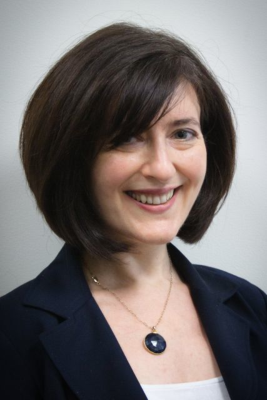
\includegraphics[height=100px]{content/day2/kuperberg-headshot.pdf}
\end{center}

\noindent
{\bfseries Abstract:} It is well established that we draw upon our real-world knowledge to predict
upcoming events and even individual words. I will discuss evidence that the neurocognitive
mechanisms that we engage in retrieving conceptual information associated with incoming words are
quite distinct from those engaged when these predictions are disconfirmed by the input. Drawing
broad links with computational models conceptualizing language comprehension as an incremental
process of belief updating, I will suggest that the engagement of these distinct neurocognitive
systems allows for comprehension that is both highly efficient and highly flexible (1).

I will first discuss studies using event-related potentials (ERPs) to examine online brain activity
during sentence and discourse comprehension. I will then draw some (still tentative) links between
this ERP literature and some relevant fMRI and MEG studies. Finally, I will discuss the advantages
of a predictive comprehension system. Predicting correctly clearly offers advantages in terms of
computational efficiency. Here I will argue that the costs incurred when we predict incorrectly are
also crucial for successful and flexible comprehension. Neurocognitive responses triggered by
prediction errors may rescue us from interpretation errors in noisy environments, may allow us learn
novel events, and may enable us to flexibly adjust our comprehension strategies in response to
everchanging task and environmental demands.

\vspace{3em}\par 

\vfill
\noindent
{\bfseries Biography}: Gina R Kuperberg is a Cognitive Neuroscientist and a Professor in the
Department of Psychology and the Cognitive Science Center at Tufts University, Boston. She is also a
Board Certified Psychiatrist and a Principal Investigator in the Psychiatry Neuroscience Program at
Massachusetts General Hospital, Harvard Medical School. Her research program aims to understand the
neurocognitive mechanisms by which the human brain builds meaning from language, and how these
mechanisms break down in neuropsychiatric disorders, particularly schizophrenia.

Dr.\ Kuperberg's Lab is situated across in both the Department of Psychology at Tufts and the
Martinos Center for Biomedical Imaging at Massachusetts General Hospital. The Lab uses multimodal
neuroimaging methods –– event-related potentials (ERPs), functional MRI (fMRI) and
magneto-encephalography (MEG) –– to probe both the spatial and temporal dimensions of cognition in
the brain. Her research program is funded by an RO1 from the National Institute of Mental Health
(NIMH), as well as awards from the Brain and Behavior Research Foundation and the Sidney Baer
Trust. She, her students, postdocs and collaborators publish in a wide range of journals of
Cognitive Neuroscience, Psycholinguistics, Experimental Psychology, Neuroimaging and Psychiatry.

Dr.\ Kuperberg has served as a standing member for the Language and Communication Study Section for
the National Institute of Health, and as a committee representative for Language for the Cognitive
Neuroscience society. Her research accomplishments have been recognized by several awards, including
the A.E. Bennett Research Award from the Society for Biological Psychiatry, the Joseph Zubin Award
for Significant Contributions to Research in Psychopathology, and an Award from Brain Research for
their most highly cited article, for her review of the architecture of the language system, Neural
Mechanisms of Language Comprehension: Challenges to Syntax.

Dr.\ Kuperberg earned her MD at St. Bartholomew's Medical School, London, and her PhD in Psychology
and Cognitive Neuroscience at Kings College, University of London. She completed an internship at
St. Bartholomew's Hospital and residency training in Psychiatry at the Maudsley Hospital and
Institute of Psychiatry, London. In 1998, she came to Boston where she completed research
fellowships in Neuroimaging and Cognitive Electrophysiology at Massachusetts General Hospital,
Harvard Medical School and Tufts University, working with David Caplan, Anders Dale and Phil
Holcomb.
\newpage
\newpage

%\section{Oral Presentations}
\vspace{1em}\par\centerline{\bfseries\Large Paper Abstracts}\vspace{1em}\par
\addcontentsline{toc}{section}{Paper Abstracts}
\paperabstract{Monday}{10:40am--11:05am}{\Btitle}{\MOaLoc}{main-268}
\paperabstract{Monday}{11:05am--11:30am}{\Btitle}{\MOaLoc}{main-319}
\paperabstract{Monday}{11:30am--11:55am}{\Btitle}{\MOaLoc}{main-276}
\paperabstract{Monday}{11:55am--12:20pm}{\Btitle}{\MOaLoc}{main-419}
\paperabstract{Monday}{10:40am--11:05am}{\Btitle}{\MObLoc}{main-441}
\paperabstract{Monday}{11:05am--11:30am}{\Btitle}{\MObLoc}{main-282}
\paperabstract{Monday}{11:30am--11:55am}{\Btitle}{\MObLoc}{main-174}
\paperabstract{Monday}{11:55am--12:20pm}{\Btitle}{\MObLoc}{main-125}
\paperabstract{Monday}{10:40am--11:05am}{\Btitle}{\MOcLoc}{main-377}
\paperabstract{Monday}{11:05am--11:30am}{\Btitle}{\MOcLoc}{main-474}
\paperabstract{Monday}{11:30am--11:55am}{\Btitle}{\MOcLoc}{main-082}
\paperabstract{Monday}{11:55am--12:20pm}{\Btitle}{\MOcLoc}{main-370}

\paperabstract{Monday}{2:00pm--2:25pm}{\Btitle}{\MTcLoc}{main-363}
\paperabstract{Monday}{2:25pm--2:50pm}{\Btitle}{\MTcLoc}{main-429}
\paperabstract{Monday}{2:50pm--3:15pm}{\Btitle}{\MTcLoc}{main-438}
\paperabstract{Monday}{3:15pm--3:40pm}{\Btitle}{\MTcLoc}{main-361}

\newpage

% I'm bypassing the \section command here because I didn't like the layout
% from the ACL-IJNLP handbook that I started from. UG
\vspace{1em}\par\centerline{\bfseries\Large Poster and Demo Session}\vspace{1em}\par
\addcontentsline{toc}{section}{Poster and Demo Session}

\noindent
\vspace{1em}\par\centerline{\bfseries NAACL HLT Demos}\vspace{1em}\par

\noindent
\paperabstract{Monday}{6:00pm--9:00pm}{Poster Session}{\PosterSessionLoc}{main-180}\par
\paperabstract{Monday}{6:00pm--9:00pm}{Poster Session}{\PosterSessionLoc}{main-393}\par
\paperabstract{Monday}{6:00pm--9:00pm}{Poster Session}{\PosterSessionLoc}{main-345}\par
\paperabstract{Monday}{6:00pm--9:00pm}{Poster Session}{\PosterSessionLoc}{main-108}\par
\paperabstract{Monday}{6:00pm--9:00pm}{Poster Session}{\PosterSessionLoc}{main-195}\par
\paperabstract{Monday}{6:00pm--9:00pm}{Poster Session}{\PosterSessionLoc}{main-410}\par
\paperabstract{Monday}{6:00pm--9:00pm}{Poster Session}{\PosterSessionLoc}{main-020}\par
\paperabstract{Monday}{6:00pm--9:00pm}{Poster Session}{\PosterSessionLoc}{main-206}\par
\paperabstract{Monday}{6:00pm--9:00pm}{Poster Session}{\PosterSessionLoc}{main-089}\par
\paperabstract{Monday}{6:00pm--9:00pm}{Poster Session}{\PosterSessionLoc}{main-420}\par
\paperabstract{Monday}{6:00pm--9:00pm}{Poster Session}{\PosterSessionLoc}{main-002}\par
\paperabstract{Monday}{6:00pm--9:00pm}{Poster Session}{\PosterSessionLoc}{main-289}\par
\paperabstract{Monday}{6:00pm--9:00pm}{Poster Session}{\PosterSessionLoc}{main-184}\par
\paperabstract{Monday}{6:00pm--9:00pm}{Poster Session}{\PosterSessionLoc}{main-293}\par
\paperabstract{Monday}{6:00pm--9:00pm}{Poster Session}{\PosterSessionLoc}{main-120}\par
\paperabstract{Monday}{6:00pm--9:00pm}{Poster Session}{\PosterSessionLoc}{main-390}\par
\paperabstract{Monday}{6:00pm--9:00pm}{Poster Session}{\PosterSessionLoc}{main-431}\par
\paperabstract{Monday}{6:00pm--9:00pm}{Poster Session}{\PosterSessionLoc}{main-137}\par
\paperabstract{Monday}{6:00pm--9:00pm}{Poster Session}{\PosterSessionLoc}{main-457}\par
\paperabstract{Monday}{6:00pm--9:00pm}{Poster Session}{\PosterSessionLoc}{main-336}\par
\paperabstract{Monday}{6:00pm--9:00pm}{Poster Session}{\PosterSessionLoc}{main-402}\par
\paperabstract{Monday}{6:00pm--9:00pm}{Poster Session}{\PosterSessionLoc}{main-075}\par
\paperabstract{Monday}{6:00pm--9:00pm}{Poster Session}{\PosterSessionLoc}{main-385}\par
\paperabstract{Monday}{6:00pm--9:00pm}{Poster Session}{\PosterSessionLoc}{main-300}\par
\paperabstract{Monday}{6:00pm--9:00pm}{Poster Session}{\PosterSessionLoc}{main-128}\par
\paperabstract{Monday}{6:00pm--9:00pm}{Poster Session}{\PosterSessionLoc}{main-264}\par
\paperabstract{Monday}{6:00pm--9:00pm}{Poster Session}{\PosterSessionLoc}{main-278}\par
\paperabstract{Monday}{6:00pm--9:00pm}{Poster Session}{\PosterSessionLoc}{main-397}\par
\paperabstract{Monday}{6:00pm--9:00pm}{Poster Session}{\PosterSessionLoc}{main-212}\par
\paperabstract{Monday}{6:00pm--9:00pm}{Poster Session}{\PosterSessionLoc}{main-250}\par
\paperabstract{Monday}{6:00pm--9:00pm}{Poster Session}{\PosterSessionLoc}{main-313}\par
\paperabstract{Monday}{6:00pm--9:00pm}{Poster Session}{\PosterSessionLoc}{main-351}\par
\paperabstract{Monday}{6:00pm--9:00pm}{Poster Session}{\PosterSessionLoc}{main-225}\par
\paperabstract{Monday}{6:00pm--9:00pm}{Poster Session}{\PosterSessionLoc}{main-340}\par
\paperabstract{Monday}{6:00pm--9:00pm}{Poster Session}{\PosterSessionLoc}{main-023}\par
\paperabstract{Monday}{6:00pm--9:00pm}{Poster Session}{\PosterSessionLoc}{main-446}\par
\paperabstract{Monday}{6:00pm--9:00pm}{Poster Session}{\PosterSessionLoc}{main-004}\par
\paperabstract{Monday}{6:00pm--9:00pm}{Poster Session}{\PosterSessionLoc}{main-372}\par
\paperabstract{Monday}{6:00pm--9:00pm}{Poster Session}{\PosterSessionLoc}{main-066}\par
\paperabstract{Monday}{6:00pm--9:00pm}{Poster Session}{\PosterSessionLoc}{main-449}\par
\paperabstract{Monday}{6:00pm--9:00pm}{Poster Session}{\PosterSessionLoc}{main-095}\par
\paperabstract{Monday}{6:00pm--9:00pm}{Poster Session}{\PosterSessionLoc}{main-057}\par
\paperabstract{Monday}{6:00pm--9:00pm}{Poster Session}{\PosterSessionLoc}{main-283}\par
\paperabstract{Monday}{6:00pm--9:00pm}{Poster Session}{\PosterSessionLoc}{main-275}\par
\paperabstract{Monday}{6:00pm--9:00pm}{Poster Session}{\PosterSessionLoc}{main-467}\par
\paperabstract{Monday}{6:00pm--9:00pm}{Poster Session}{\PosterSessionLoc}{main-070}\par
\paperabstract{Monday}{6:00pm--9:00pm}{Poster Session}{\PosterSessionLoc}{main-221}\par
\paperabstract{Monday}{6:00pm--9:00pm}{Poster Session}{\PosterSessionLoc}{main-072}\par



\posterentry{demo-001}\\[1ex]
\posterentry{demo-002}\\[1ex]
\posterentry{demo-004}\\[1ex]
\posterentry{demo-006}\\[1ex]
\posterentry{demo-008}\\[1ex]
\posterentry{demo-009}\\[1ex]
\posterentry{demo-012}\\[1ex]
\posterentry{demo-015}\\[1ex]
\posterentry{demo-016}\\[1ex]


\noindent
\vspace{1em}\par\centerline{\bfseries Posters from the Student Research Workshop}\vspace{1em}\par

\noindent
\posterentry{srw-005}\\[1ex]
\posterentry{srw-020}\\[1ex]
\posterentry{srw-008}\\[1ex]
\posterentry{srw-007}\\[1ex]
\posterentry{srw-002}\\[1ex]
\posterentry{srw-010}\\[1ex]
\posterentry{srw-018}\\[1ex]
\posterentry{srw-015}\\[1ex]
\posterentry{srw-024}\\[1ex]
\posterentry{srw-016}\\[1ex]
\posterentry{srw-014}\\[1ex]
\posterentry{srw-012}\\[1ex]
\posterentry{srw-021}\\[1ex]

\input{auto/srw/monday-srw-2.tex}

\noindent
\vspace{1em}\par\centerline{\bfseries NAACL HLT Posters}\vspace{1em}\par

\noindent
\posterentry{main-180}\\[1ex]
\posterentry{main-393}\\[1ex]
\posterentry{main-345}\\[1ex]
\posterentry{main-108}\\[1ex]
\posterentry{main-195}\\[1ex]
\posterentry{main-410}\\[1ex]
\posterentry{main-020}\\[1ex]
\posterentry{main-206}\\[1ex]
\posterentry{main-089}\\[1ex]
\posterentry{main-420}\\[1ex]
\posterentry{main-002}\\[1ex]
\posterentry{main-289}\\[1ex]
\posterentry{main-184}\\[1ex]
\posterentry{main-293}\\[1ex]
\posterentry{main-120}\\[1ex]
\posterentry{main-390}\\[1ex]
\posterentry{main-431}\\[1ex]
\posterentry{main-137}\\[1ex]
\posterentry{main-457}\\[1ex]
\posterentry{main-336}\\[1ex]
\posterentry{main-402}\\[1ex]
\posterentry{main-075}\\[1ex]
\posterentry{main-385}\\[1ex]
\posterentry{main-300}\\[1ex]
\posterentry{main-128}\\[1ex]
\posterentry{main-264}\\[1ex]
\posterentry{main-278}\\[1ex]
\posterentry{main-397}\\[1ex]
\posterentry{main-212}\\[1ex]
\posterentry{main-250}\\[1ex]
\posterentry{main-313}\\[1ex]
\posterentry{main-351}\\[1ex]
\posterentry{main-225}\\[1ex]
\posterentry{main-340}\\[1ex]
\posterentry{main-023}\\[1ex]
\posterentry{main-446}\\[1ex]
\posterentry{main-004}\\[1ex]
\posterentry{main-372}\\[1ex]
\posterentry{main-066}\\[1ex]
\posterentry{main-449}\\[1ex]
\posterentry{main-095}\\[1ex]
\posterentry{main-057}\\[1ex]
\posterentry{main-283}\\[1ex]
\posterentry{main-275}\\[1ex]
\posterentry{main-467}\\[1ex]
\posterentry{main-070}\\[1ex]
\posterentry{main-221}\\[1ex]
\posterentry{main-072}\\[1ex]

\input{auto/main/monday-main-4.tex}

\noindent
\vspace{1em}\par\centerline{\bfseries\Large Demo and Poster Abstracts}\vspace{1em}\par
\addcontentsline{toc}{section}{Demo and Poster Abstracts}
\input{auto/demo/monday-demo-1-Demo-abstracts.tex}
\input{auto/srw/monday-srw-1-RP-abstracts.tex}
\input{auto/srw/monday-srw-2-TP-abstracts.tex}
\input{auto/main/monday-main-3-MonP-abstracts.tex}
\input{auto/main/monday-main-4-MonPS-abstracts.tex}

